\par El problema se basa en calcular el camino de mínima longitud que debe recorrer un jugador para pasar por una serie de nodos ubicados en un mapa, cumpliendo con ciertas condiciones que mencionaremos a continuación. Los nodos pueden ser de dos tipos: Paradas o Gimnasios. Cada nodo cuenta con una ubicación, expresada en función de sus coordenadas \textit{x} e \textit{y}. Para poder ir a un nodo del tipo Gimnasio (en adelante \textit{G}) se debe contar con una cierta cantidad de pociones. Estas pociones son obtenidas al pasar por un nodo del tipo Parada (en adelante \textit{P}). Al ir a un nodo P el jugador obtiene 3 pociones. El jugador cuenta con una mochila con una cierta capacidad (que limita la cantidad de pociones que puede llevar). En caso de que un jugador exceda su límite en la mochila deberá descartar las pociones sobrantes (que no se podrán utilizar mas). Es importante marcar que un jugador no puede pasar mas de una vez por ningún nodo (de cualquier tipo). El objetivo del jugador es recorrer en la menor distancia posible todos los nodos G.

\par Cabe destacar que la distancia entre dos nodos será la distancia Euclediana. Por lo que, dados dos nodos $N_1 = (x_1, y_1)$ y $N_2 = (x_2, y_2)$:

\begin{equation}
	dist(N_1, N_2) = \sqrt{ (x_1 - x_2)^2 + (y_1 - y_2)^2}
\end{equation}

\par En resumen, tenemos que un jugador debe pasar por todos los nodos G en la menor distancia posible. Para ello debe pasar también por nodos P para recargar pociones (siempre que no exceda el límite de su mochila).

\begin{figure}[h]
	\begin{center}
		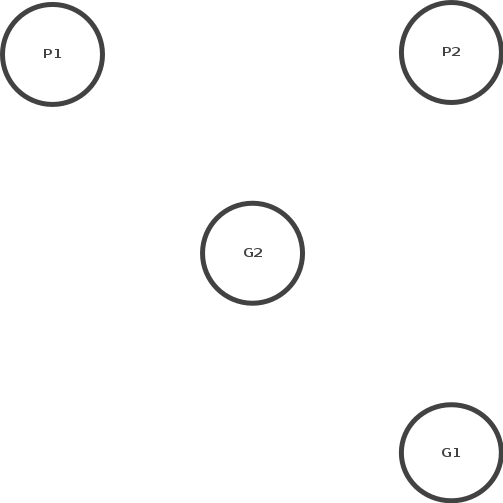
\includegraphics[width=0.5\textwidth]{img/descripcion/descripcion_ejemplo_entrada.png}
		\caption{Mapa de entrada ejemplo.}
		\label{fig: descripcion_ejemplo_entrada}
	\end{center}
\end{figure}

\par En la figura \ref{fig: descripcion_ejemplo_entrada} podemos ver un mapa que corresponde a un ejemplo de datos de entrada del problema. Veamos en detalle este ejemplo. Tenemos una mochila con capacidad 5 y dos nodos P y dos nodos G con las siguientes características:

\begin{itemize}
	\item $P_1$: nodo P ubicado en (2, 1).
	\item $P_2$: nodo P ubicado en (2, 3).
	\item $G_2$: nodo G ubicado en (4, 3) y con cantidad de pociones necesarias igual a 3.
	\item $G_2$: nodo G ubicado en (3, 2) y con cantidad de pociones necesarias igual a 2.
\end{itemize}

\par Para este caso en particular, el camino mas corto es el que se muestra en la figura \ref{fig: descripcion_ejemplo_solucion}. Podemos ver que el camino comienza en el nodo $P_1$ donde obtiene 3 pociones, va hacia el nodo $G_2$, donde pierde 3 pociones y queda sin ninguna; luego hacia el nodo $P_2$, donde obtiene 3 pociones; y finaliza en el nodo $G_1$, perdiendo 2 pociones y quedando sólo con una. En la figura vemos también que están detalladas las distancias entre los nodos del camino. Finalmente, este camino nos da una distancia total de 4.82842 y es una solución al problema.

\begin{figure}[h]
	\begin{center}
		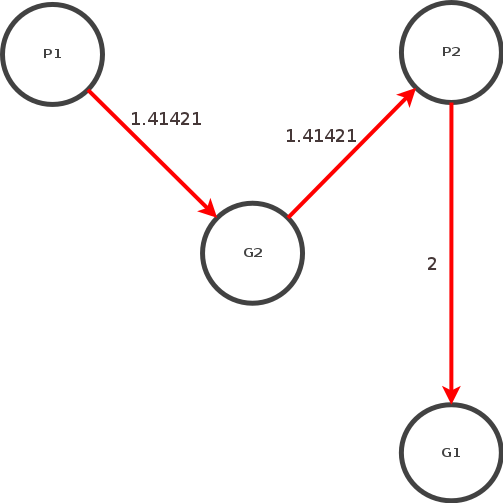
\includegraphics[width=0.4\textwidth]{img/descripcion/descripcion_ejemplo_solucion.png}
		\caption{Mapa de entrada ejemplo con el camino solución marcado.}
		\label{fig: descripcion_ejemplo_solucion}
	\end{center}
\end{figure}

\par En este informe se van a presentar distintos tipos de algoritmos para resolver este problema. En primer lugar, un algoritmo exacto. Luego, algoritmos basados en heurísticas y metaheurísticas. Se compararán los distintos algoritmos para determinar cuál responde mejor al problema planteado en función de tiempos y precisión de la solución.